% !TEX root = task-3-10-4.tex
% Editable task bank. Append new BankTask blocks at the end of the document.
\documentclass[12pt,a4paper]{article}
\usepackage{physics-textbook}
\usepackage{graphicx,needspace}
\usetikzlibrary{decorations.pathmorphing}
\newif\ifShowSolutions
\ifdefined\TutorEdition
  \ShowSolutionstrue
\else
  \ShowSolutionsfalse % Change to \ShowSolutionstrue to display solutions.
\fi
\newcounter{banktask}
\newsavebox{\BankTaskBox}
\newcommand{\BankTaskContent}[3]{%
  \noindent\textbf{\thebanktask.}\quad #2\par
  \ifShowSolutions
    \Needspace{50mm}% Keep the solution heading with its opening text or diagram.
    #3\par
    \ifdefined\TutorEdition
      \ifcsname TutorSource#1\endcsname
        \nopagebreak\smallskip{\small\csname TutorSource#1\endcsname\par}%
      \fi
    \fi
  \fi
}
\newcommand{\BankTask}[3]{%
  \refstepcounter{banktask}\par\medskip
  \sbox{\BankTaskBox}{\begin{minipage}{\linewidth}%
    \BankTaskContent{#1}{#2}{#3}\end{minipage}}%
  \ifdim\dimexpr\ht\BankTaskBox+\dp\BankTaskBox\relax>\dimexpr\textheight-20mm\relax
    \Needspace{35mm}\BankTaskContent{#1}{#2}{#3}%
  \else
    \Needspace{\dimexpr\ht\BankTaskBox+\dp\BankTaskBox\relax}%
    \noindent\usebox{\BankTaskBox}\par
  \fi
  \medskip
}
\begin{document}
\BookSubsection{3.10.4}{Смешанное соединение}


% Source F934C0: https://ege.fipi.ru/bank/questions.php?search=1&proj=BA1F39653304A5B041B656915DC36B38&qid=F934C0
\BankTask{F934C0}{
На участке цепи, изображённом на рисунке, сопротивление каждого из четырёх резисторов равно $6\,\text{Ом}$. Каково общее сопротивление цепи между клеммами $\text{А}$ и $\text{В}$?
\begin{center}
\begin{tikzpicture}[x=1cm,y=1cm,>=stealth,line width=0.8pt]
\draw (0,0) circle (0.06) node[left=4pt] {$\text{А}$};
\draw (0.06,0)--(0.8,0);
\draw (0.8,0)--(0.8,0.35)--(1.05,0.35);
\draw (1.05,0.18) rectangle (1.85,0.52);
\draw (1.85,0.35)--(2.1,0.35)--(2.1,0);
\draw (0.8,0)--(0.8,-0.35)--(1.05,-0.35);
\draw (1.05,-0.52) rectangle (1.85,-0.18);
\draw (1.85,-0.35)--(2.1,-0.35)--(2.1,0);
\fill (0.8,0) circle (0.055);
\fill (2.1,0) circle (0.055);
\draw (2.1,0)--(2.8,0);
\draw (2.8,-0.17) rectangle (3.6,0.17);
\draw (3.6,0)--(4.3,0);
\draw (4.3,-0.17) rectangle (5.1,0.17);
\draw (5.1,0)--(5.84,0);
\draw (5.9,0) circle (0.06) node[right=4pt] {$\text{В}$};
\end{tikzpicture}
\end{center} (в $\text{Ом}$).
}{
\smallskip\noindent\textbf{Решение от GPT}\par
Два левых резистора соединены параллельно, остальные — последовательно с ними:
\[
R_{\text{общ}}=\frac{6\cdot6}{6+6}+6+6=15\ \text{Ом}.
\]
Ответ: \(15\,\text{Ом}\).
}

% Source 849501: https://ege.fipi.ru/bank/questions.php?search=1&proj=BA1F39653304A5B041B656915DC36B38&qid=849501
\BankTask{849501}{
\begin{center}
\begin{tikzpicture}[x=1cm,y=1cm,>=stealth,line width=0.8pt]
\draw (0,1.6) circle (0.06) node[left=4pt] {$\text{А}$};
\draw (0.06,1.6)--(0.5,1.6);
\draw (0.5,1.43) rectangle (1.3,1.77);
\node[above] at (0.9,1.77) {\(R\)};
\draw (1.3,1.6)--(1.7,1.6)--(3.3,1.6)--(3.3,1.3);
\draw (1.7,1.6)--(1.7,1.3);
\draw (1.53,0.3) rectangle (1.87,1.3);
\node[left] at (1.53,0.8) {\(R\)};
\draw (1.7,0.3)--(1.7,0);
\draw (3.13,0.3) rectangle (3.47,1.3);
\node[right] at (3.47,0.8) {\(R\)};
\draw (3.3,0.3)--(3.3,0)--(0.06,0);
\draw (0,0) circle (0.06) node[left=4pt] {$\text{В}$};
\draw (1.7,1.6)--(2.35,0.95);
\draw (2.35,0.95)--(2.85,0.9);
\draw (2.65,0.65)--(3.3,0);
\node at (2.55,1.17) {$\text{К}$};
\fill (1.7,1.6) circle (0.045);
\fill (1.7,0) circle (0.045);
\fill (3.3,0) circle (0.045);
\end{tikzpicture}
\end{center}
На сколько уменьшится сопротивление участка цепи $\text{АВ}$, изображённого на рисунке, если ключ $\text{К}$ замкнуть? Сопротивление каждого резистора $R=2\,\text{Ом}$ (в $\text{Ом}$).
}{
\smallskip\noindent\textbf{Решение от GPT}\par
При разомкнутом ключе два вертикальных резистора соединены параллельно:
\[
R_{\text{разомк}}=R+\frac{R}{2}=3\ \text{Ом}.
\]
Замкнутый ключ закорачивает оба вертикальных резистора, поэтому \(R_{\text{замк}}=R=2\ \text{Ом}\). Уменьшение сопротивления:
\[
\Delta R=3-2=1\ \text{Ом}.
\]
Ответ: \(1\,\text{Ом}\).
}

% Source A5D05E: https://ege.fipi.ru/bank/questions.php?search=1&proj=BA1F39653304A5B041B656915DC36B38&qid=A5D05E
\BankTask{A5D05E}{
Сопротивление каждого резистора в схеме участка цепи на рисунке равно $100\,\text{Ом}$. Участок подключён к источнику постоянного напряжения выводами $A$ и $B$. Напряжение на резисторе $R_2$ равно $12\,\text{В}$. Чему равно напряжение на резисторе $R_3$?
\begin{center}
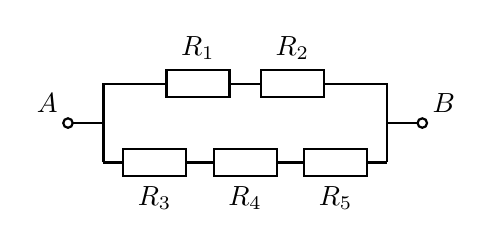
\begin{tikzpicture}[x=1cm,y=1cm,>=stealth,line width=0.8pt]
\draw (0,0) circle (0.06) node[above left] {\(A\)};
\draw (0.06,0)--(0.45,0);
\draw (0.45,-0.5)--(0.45,0.5)--(1.25,0.5);
\draw (1.25,0.33) rectangle (2.05,0.67);
\node[above] at (1.65,0.67) {\(R_1\)};
\draw (2.05,0.5)--(2.45,0.5);
\draw (2.45,0.33) rectangle (3.25,0.67);
\node[above] at (2.85,0.67) {\(R_2\)};
\draw (3.25,0.5)--(4.05,0.5)--(4.05,-0.5);
\draw (0.45,-0.5)--(0.7,-0.5);
\draw (0.7,-0.67) rectangle (1.5,-0.33);
\node[below] at (1.1,-0.67) {\(R_3\)};
\draw (1.5,-0.5)--(1.85,-0.5);
\draw (1.85,-0.67) rectangle (2.65,-0.33);
\node[below] at (2.25,-0.67) {\(R_4\)};
\draw (2.65,-0.5)--(3,-0.5);
\draw (3,-0.67) rectangle (3.8,-0.33);
\node[below] at (3.4,-0.67) {\(R_5\)};
\draw (3.8,-0.5)--(4.05,-0.5);
\draw (4.05,0)--(4.44,0);
\draw (4.5,0) circle (0.06) node[above right] {\(B\)};
\end{tikzpicture}
\end{center} (в $\text{В}$).
}{
\smallskip\noindent\textbf{Решение от GPT}\par
В верхней ветви два одинаковых последовательных резистора, поэтому
\[
U_{AB}=2U_2=24\ \text{В}.
\]
На нижней ветви такое же напряжение, которое делится поровну между тремя одинаковыми резисторами:
\[
U_3=\frac{U_{AB}}{3}=8\ \text{В}.
\]
Ответ: \(8\,\text{В}\).
}

% Source 8D32C8: https://ege.fipi.ru/bank/questions.php?search=1&proj=BA1F39653304A5B041B656915DC36B38&qid=8D32C8
\BankTask{8D32C8}{
Через участок цепи (см. рисунок) течёт постоянный ток $I=4\,\text{А}$. Какую силу тока покажет включённый в эту цепь идеальный амперметр, если сопротивление каждого резистора $r=1\,\text{Ом}$?
\begin{center}
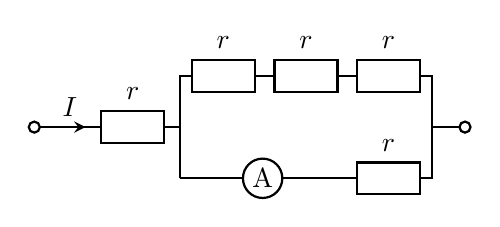
\begin{tikzpicture}[x=1cm,y=1cm,>=stealth,line width=0.8pt]
\draw (0,0) circle (0.07);
\draw (0.07,0)--(0.85,0);
\draw[->] (0.25,0)--(0.65,0) node[midway,above] {$I$};
\draw (0.85,-0.2) rectangle (1.65,0.2);
\node at (1.25,0.42) {$r$};
\draw (1.65,0)--(1.85,0);
\draw (1.85,-0.65)--(1.85,0.65)--(2,0.65);
\draw (2,0.45) rectangle (2.8,0.85);
\node at (2.4,1.07) {$r$};
\draw (2.8,0.65)--(3.05,0.65);
\draw (3.05,0.45) rectangle (3.85,0.85);
\node at (3.45,1.07) {$r$};
\draw (3.85,0.65)--(4.1,0.65);
\draw (4.1,0.45) rectangle (4.9,0.85);
\node at (4.5,1.07) {$r$};
\draw (4.9,0.65)--(5.05,0.65)--(5.05,-0.65)--(4.9,-0.65);
\draw (1.85,-0.65)--(2.65,-0.65);
\draw (2.9,-0.65) circle (0.25);
\node at (2.9,-0.65) {$\mathrm{A}$};
\draw (3.15,-0.65)--(4.1,-0.65);
\draw (4.1,-0.85) rectangle (4.9,-0.45);
\node at (4.5,-0.23) {$r$};
\draw (5.05,0)--(5.4,0);
\draw (5.47,0) circle (0.07);
\end{tikzpicture}
\end{center} (в $\text{А}$).
}{
\smallskip\noindent\textbf{Решение от GPT}\par
Сопротивления верхней и нижней параллельных ветвей равны $R_{\text{в}}=3r$ и $R_{\text{н}}=r$ (сопротивление идеального амперметра равно нулю). Поэтому $I_{\text{н}}/I_{\text{в}}=3$, а $I_{\text{н}}+I_{\text{в}}=I$. Показание амперметра:
\[
I_A=\frac{3}{4}I=3\,\text{А}.
\]
Ответ: $3\,\text{А}$.
}

% Source D35A43: https://ege.fipi.ru/bank/questions.php?search=1&proj=BA1F39653304A5B041B656915DC36B38&qid=D35A43
\BankTask{D35A43}{
Восемь одинаковых резисторов с сопротивлением $r=1\,\text{Ом}$ соединены в электрическую цепь, через которую течёт ток $I=4\,\text{А}$ (см. рисунок). Какое напряжение (в $\text{В}$) показывает идеальный вольтметр?
\begin{center}
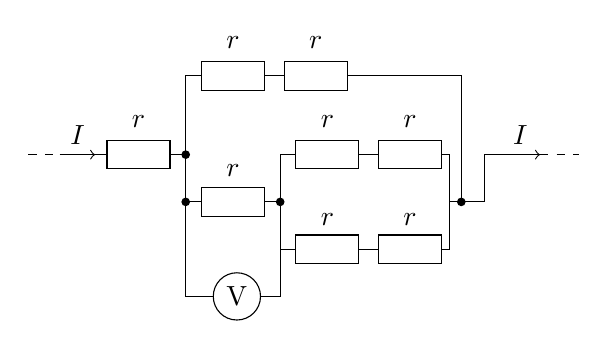
\begin{tikzpicture}[x=1cm,y=1cm]
\draw[dashed] (-1,0)--(-0.6,0);
\draw[->] (-0.6,0)--(-0.15,0) node[midway,above] {$I$};
\draw (-0.15,0)--(0,0);
\draw (0,-0.18) rectangle (0.8,0.18);
\node at (0.4,0.42) {$r$};
\draw (0.8,0)--(1,0)--(1,1)--(1.2,1);
\draw (1.2,0.82) rectangle (2,1.18);
\node at (1.6,1.42) {$r$};
\draw (2,1)--(2.25,1);
\draw (2.25,0.82) rectangle (3.05,1.18);
\node at (2.65,1.42) {$r$};
\draw (3.05,1)--(4.5,1)--(4.5,-0.6);
\draw (1,0)--(1,-0.6)--(1.2,-0.6);
\draw (1.2,-0.78) rectangle (2,-0.42);
\node at (1.6,-0.2) {$r$};
\draw (2,-0.6)--(2.2,-0.6);
\draw (2.2,-0.6)--(2.2,0)--(2.4,0);
\draw (2.4,-0.18) rectangle (3.2,0.18);
\node at (2.8,0.42) {$r$};
\draw (3.2,0)--(3.45,0);
\draw (3.45,-0.18) rectangle (4.25,0.18);
\node at (3.85,0.42) {$r$};
\draw (4.25,0)--(4.35,0)--(4.35,-0.6)--(4.5,-0.6);
\draw (2.2,-0.6)--(2.2,-1.2)--(2.4,-1.2);
\draw (2.4,-1.38) rectangle (3.2,-1.02);
\node at (2.8,-0.82) {$r$};
\draw (3.2,-1.2)--(3.45,-1.2);
\draw (3.45,-1.38) rectangle (4.25,-1.02);
\node at (3.85,-0.82) {$r$};
\draw (4.25,-1.2)--(4.35,-1.2)--(4.35,-0.6);
\draw (1,-0.6)--(1,-1.8)--(1.35,-1.8);
\draw (1.65,-1.8) circle (0.3);
\node at (1.65,-1.8) {$\mathrm{V}$};
\draw (1.95,-1.8)--(2.2,-1.8)--(2.2,-0.6);
\draw (4.5,-0.6)--(4.8,-0.6)--(4.8,0)--(5,0);
\draw[->] (5,0)--(5.5,0) node[midway,above] {$I$};
\draw[dashed] (5.5,0)--(6,0);
\foreach \x/\y in {1/0,1/-0.6,2.2/-0.6,4.5/-0.6} \fill (\x,\y) circle (0.055);
\end{tikzpicture}
\end{center}
}{
\smallskip\noindent\textbf{Решение от GPT}\par
Идеальный вольтметр тока не проводит. Две правые ветви имеют сопротивления $2r$ каждая, поэтому их параллельное соединение имеет сопротивление $r$. Нижняя ветвь между левым и правым узлами имеет сопротивление $r+r=2r$, верхняя — также $2r$. Ток делится поровну. Через резистор, к которому подключён вольтметр, течёт $I/2$:
\[
U=\frac{I}{2}r=\frac{4}{2}\cdot1=2\,\text{В}.
\]
}

% Source 38951: https://phys-ege.sdamgia.ru/problem?id=38951
\BankTask{38951}{
Три одинаковых резистора и два одинаковых идеальных диода включены в электрическую цепь, показанную на рисунке, и подключены к аккумулятору в точках В и С. Показания амперметра равны $2\,\text{А}$. Определите силу тока через амперметр при смене полярности подключения аккумулятора. Нарисуйте эквивалентные электрические схемы для двух случаев подключения аккумулятора. Опираясь на законы электродинамики, поясните свой ответ. Сопротивлением амперметра и внутренним сопротивлением аккумулятора пренебречь.
\begin{center}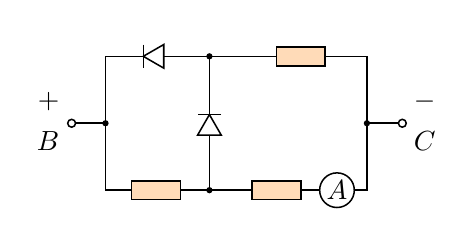
\begin{tikzpicture}[>=stealth,line width=.55pt]\draw(.5,.85)--(.88,.85) (.88,0)--(.88,1.7)--(4.2,1.7)--(4.2,0)--(.88,0) (4.2,.85)--(4.6,.85) (2.2,0)--(2.2,1.7);\fill(.88,.85)circle(.04) (4.2,.85)circle(.04) (2.2,0)circle(.04) (2.2,1.7)circle(.04);\draw(.45,.85)circle(.05) (4.65,.85)circle(.05);\node[left]at(.42,1.13){$+$};\node[left]at(.42,.63){$B$};\node[right]at(4.67,1.13){$-$};\node[right]at(4.67,.63){$C$};\begin{scope}[shift={(1.47,1.7)},rotate=180]\draw[fill=white](-.15,-.15)--(.11,0)--(-.15,.15)--cycle;\draw(.11,-.15)--(.11,.15);\end{scope}\begin{scope}[shift={(2.2,0.85)},rotate=90]\draw[fill=white](-.15,-.15)--(.11,0)--(-.15,.15)--cycle;\draw(.11,-.15)--(.11,.15);\end{scope}\draw[fill=orange!28](3.05,1.58)rectangle(3.67,1.8199999999999998);\node[above]at(3.36,1.8199999999999998){$$};\draw[fill=orange!28](1.21,-0.12)rectangle(1.83,0.12);\node[above]at(1.52,0.12){$$};\draw[fill=orange!28](2.7399999999999998,-0.12)rectangle(3.36,0.12);\node[above]at(3.05,0.12){$$};\draw[fill=white](3.82,0)circle(.22)node{$A$};\end{tikzpicture}\end{center}
}{
\smallskip\noindent\textbf{Решение}\par
При первом подключении цепи к источнику постоянного напряжения ток через верхний диод не проходит, через второй диод  — проходит, при этом точки, между которыми он находится, имеют равные потенциалы. Тогда эквивалентная схема имеет вид, изображенный на рис. $1$. Так как при параллельном соединении резисторы имеют одинаковое сопротивление, а амперметр идеальный, то через обе ветки идет ток, равный $2\,\text{А}$, а в неразветвленном участке цепи сила тока $I=I_1 + I_2=4\,\text{А}.$ Учитывая законы последовательного и параллельного соединения проводников, находим общее сопротивление цепи:   $R_{\,\text{общ}}= \frac{3R}{2} .$ Так как внутренним сопротивлением аккумулятора можно пренебречь, то напряжение на его клеммах равно по закону Ома $U=IR_{\,\text{общ}}=4 \cdot \frac{3R}{2} =6R.$
При изменении полярности подключения источника напряжения ток пройдет через оба диода, поэтому ток через левый резистор не пойдет. В этом случае получаем эквивалентную схему, изображенную на рис. $2$.
В цепи имеется два резистора, соединенные параллельно. Поэтому общее сопротивление цепи станет равным $R'_{\,\text{общ}}= \frac{R}{2} ,$ а общая сила тока $I'= \frac{U}{R'_{\,\text{общ}}} =12\,\text{А}.$ Так как обе ветви параллельно соединенных участков имеют одинаковое сопротивление, то ток через резистор и амперметр будет равен $I_A= \frac{I'}{2} = \frac{12}{2} =6\,\text{А}.$

\begin{center}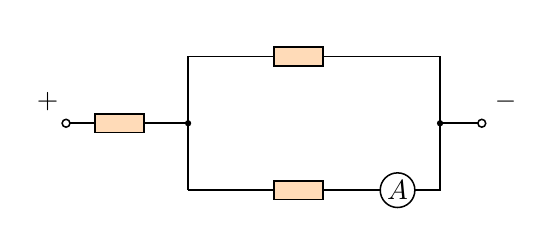
\begin{tikzpicture}[>=stealth,line width=.55pt]\draw(1,0)--(1,1.7)--(4.2,1.7)--(4.2,0)--(1,0);\fill(1,.85)circle(.04) (4.2,.85)circle(.04);\draw(4.2,.85)--(4.68,.85);\draw(4.73,.85)circle(.05);\draw(-.5,.85)--(1,.85);\draw(-.55,.85)circle(.05);\node[left]at(-.52,1.13){$+$};\node[right]at(4.77,1.13){$-$};\draw[fill=orange!28](-0.18,0.73)rectangle(0.44,0.97);\node[above]at(0.13,0.97){$$};\draw[fill=orange!28](2.09,1.58)rectangle(2.71,1.8199999999999998);\node[above]at(2.4,1.8199999999999998){$$};\draw[fill=orange!28](2.09,-0.12)rectangle(2.71,0.12);\node[above]at(2.4,0.12){$$};\draw[fill=white](3.66,0)circle(.22)node{$A$};\end{tikzpicture}\end{center}
Рис. $1$

\begin{center}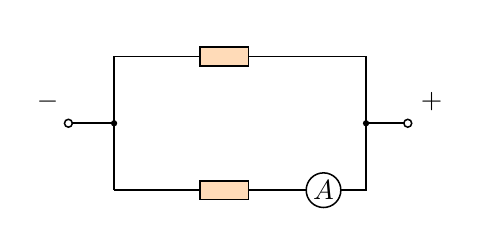
\begin{tikzpicture}[>=stealth,line width=.55pt]\draw(1,0)--(1,1.7)--(4.2,1.7)--(4.2,0)--(1,0);\fill(1,.85)circle(.04) (4.2,.85)circle(.04);\draw(4.2,.85)--(4.68,.85);\draw(4.73,.85)circle(.05);\draw(.47,.85)--(1,.85);\draw(.42,.85)circle(.05);\node[left]at(.42,1.13){$-$};\node[right]at(4.77,1.13){$+$};\draw[fill=orange!28](2.09,1.58)rectangle(2.71,1.8199999999999998);\node[above]at(2.4,1.8199999999999998){$$};\draw[fill=orange!28](2.09,-0.12)rectangle(2.71,0.12);\node[above]at(2.4,0.12){$$};\draw[fill=white](3.66,0)circle(.22)node{$A$};\end{tikzpicture}\end{center}
Рис. $2$

Ответ: сила тока через амперметр станет равной $6\,\text{А}$.
}

% Source 4963: https://phys-ege.sdamgia.ru/problem?id=4963
\BankTask{4963}{
\begin{center}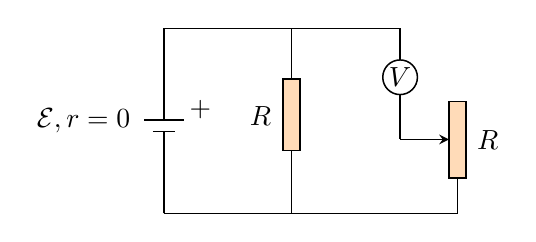
\begin{tikzpicture}[>=stealth,line width=.55pt]\draw(0,0)--(0,1.04) (0,1.19)--(0,2.35)--(3,2.35)--(3,.94) (0,0)--(3.73,0)--(3.73,1.42) (1.62,0)--(1.62,2.35);\draw(-.25,1.19)--(.25,1.19) (-.14,1.04)--(.14,1.04);\draw[->](3,.94)--(3.62,.94);\draw[fill=orange!28](1.51,.8)rectangle(1.73,1.71) (3.62,.45)rectangle(3.84,1.42);\node[left]at(-.3,1.18){$\mathcal E,r=0$};\node[right]at(.2,1.32){$+$};\node[left]at(1.49,1.24){$R$};\node[right]at(3.85,.93){$R$};\draw[fill=white](3,1.73)circle(.22)node{$V$};\end{tikzpicture}\end{center}В схеме на рисунке сопротивление резистора и полное сопротивление реостата равны R, ЭДС батарейки равна Е, ее внутреннее сопротивление ничтожно ($r = 0$). Как ведут себя (увеличиваются, уменьшаются, остаются постоянными) показания идеального вольтметра при перемещении движка реостата из крайнего верхнего в крайнее нижнее положение? Ответ поясните, указав, какие физические закономерности Вы использовали для объяснения.
}{
\smallskip\noindent\textbf{Решение}\par
Вольтметр подключают параллельно к тому участку, на котором нужно измерить напряжение. При этом, естественно, часть тока в цепи начинает течь через сам вольтметр. Тем самым вольтметр вносит возмущение в цепь и показывает напряжение, которое отличается от реального (когда вольтметра нет). Идеальным вольтметром называют прибор, который данной проблемой не страдает. То есть он имеет бесконечное собственное сопротивление. Действительно, рассмотрим положение ползунка реостата, когда он полностью выключен. При параллельном соединении напряжения совпадают:

\[I_RR=U_V=I_VR_V \Longleftrightarrow I_V= \frac{I_RR}{R_V} =0\]

При перемещении ползунка реостата к бесконечному сопротивлению вольтметра прибавляется конечное сопротивление реостата, при этом вольтметр не перестает быть идеальным, ток через него, а значит, и через реостат не течет. Полное сопротивление цепи не изменяется, а значит, полный ток в цепи также остается неизменным $( R_{\,\text{н}} = \frac{R ( R_V + R_{\,\text{р}} )}{R + R_V + R_{\,\text{р}}} =R ,$ по закону Ома для полной цепи $I= \frac{E}{R_{\,\text{н}}} ) .$) Следовательно, на сопротивлении падает одинаковое напряжение при любом положении ползунка ($U=IR$), то есть показания вольтметра не изменяются.
}

\end{document}
